\documentclass{article}

% For figures
\usepackage{graphicx} % more modern
\usepackage{subfigure} 

% For citations
% \usepackage{natbib}

% For algorithms
\usepackage{algorithm}
\usepackage{algorithmic}

\usepackage{hyperref}

% Packages hyperref and algorithmic misbehave sometimes.  We can fix
% this with the following command.
\newcommand{\theHalgorithm}{\arabic{algorithm}}

% \usepackage{sty/icml2013} 
% Employ this version of the ``usepackage'' statement after the paper has
% been accepted, when creating the final version.  This will set the
% note in the first column to ``Proceedings of the...''
\usepackage[accepted]{sty/icml2013}


% The \icmltitle you define below is probably too long as a header.
% Therefore, a short form for the running title is supplied here:
\icmltitlerunning{Clustering and Topic Discovery in Gene Expression Data}

\begin{document} 

\twocolumn[
\icmltitle{Bayesian Clustering and Topic Discovery: \\ 
           Adventures with Gene Expression Data}

% It is OKAY to include author information, even for blind
% submissions: the style file will automatically remove it for you
% unless you've provided the [accepted] option to the icml2013
% package.
\icmlauthor{Karren Dai Yang, Skanda Koppula}{\{karren, skoppula\}@mit.edu}
\icmladdress{Massachusetts Institute of Technology,
            Cambridge, MA 02139 USA}

% You may provide any keywords that you 
% find helpful for describing your paper; these are used to populate 
% the "keywords" metadata in the PDF but will not be shown in the document
\icmlkeywords{boring formatting information, machine learning, ICML}

\vskip 0.3in
]

\section{Introduction}
\label{intro}
% copied from proposal
Tumors are composed of different sub-populations of cells, and these sub-populations often exhibit shared patterns of gene expression. With contemporary sequencing machines, it is possible to obtain the expression levels of 10,000+ genes for 1000+ cells in a single experiment. 

\subsection{Prior work}
% copied from proposal
Prior research has applied basic measures of statistical distance to cluster cell groups or gene modules based on samples of single-cell RNA-sequencing (scRNA-seq) data taken from tumors \cite{nature}.  Good clustering of scRNA-seq data often has biologically meaningful results, and as such, a wide variety of correlation based methods have been used in prior work to derive meaning from scRNA-seq data \cite{coexpression, consensus, profiling}. We believe that Bayesian methods for clustering and topic modeling can be more illuminating than these previous methods, due to their consideration of higher-order relationships within the data. \\

\subsection{Description of Data}

\begin{figure}[ht]
\vskip 0.2in
\begin{center}
\centerline{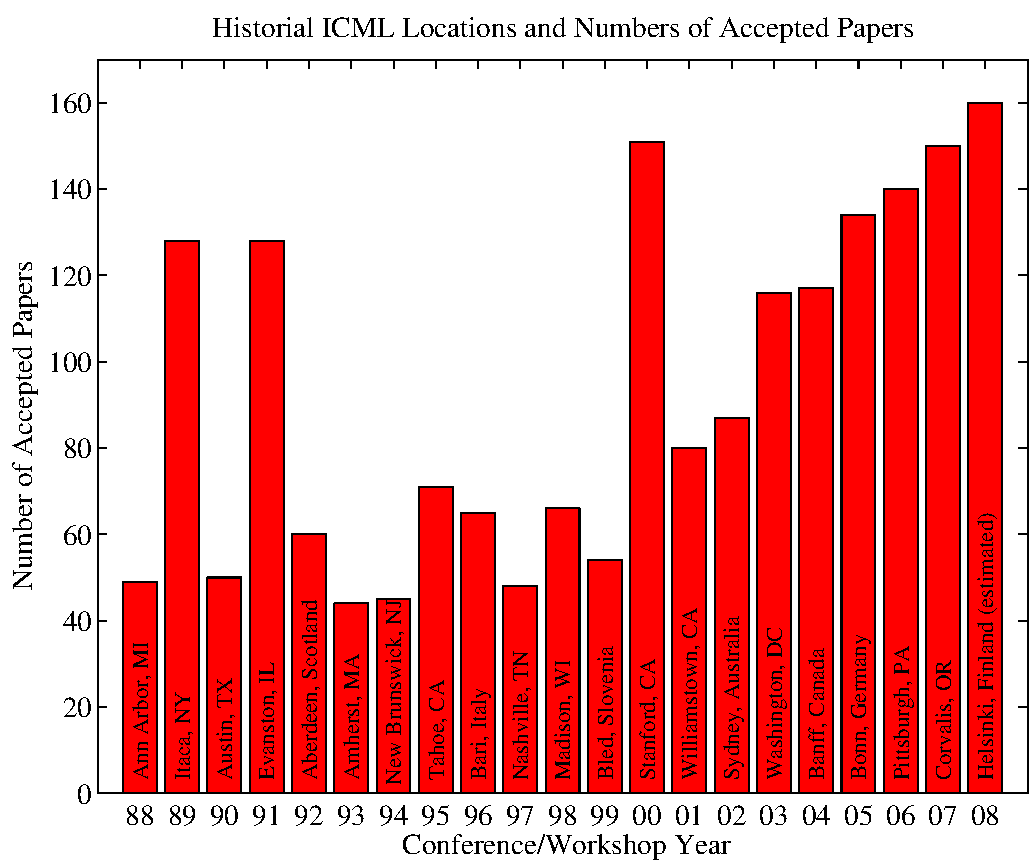
\includegraphics[width=\columnwidth]{figs/examplegraph}}
\caption{This is a demo figure.}
\label{alabel}
\end{center}
\vskip -0.2in
\end{figure} 

\subsection{Structure of Report}
% copied from proposal
In this project, we applied Bayesian methods for clustering and topic discovery to discover meaningful cell clusters and gene modules from single-cell RNA-sequencing (scRNA-seq) datasets from tumors. We first intend to explore the use of a hierarchical topic model, Latent Dirichlet Allocation (LDA) \cite{LDA}, as well as two non-parametric topic models, Hierarchical Dirichlet Processes (HDP) \cite{HDP} and the Indian Buffet Process Compound Dirichlet Process (IBP-CDP) \cite{IBP} for analyzing
scRNA-seq data. We will evaluate these models based on their ability to discover meaningful functional gene modules. Subsequently, we plan to explore the use of mixture models to cluster cells based on the output of the topic models, which we will evaluate based on their ability to differentiate cell types (e.g. immune, cancer, non-cancerous). Finally, we will train a combined clustering-topic model (e.g. MGCTM \cite{pengtao}) to see if it outperforms the individual models. We will compare the
results of these methods with standard methods used in prior work, and evaluate these methods' robustness to noise. Time permitting, we will study extensions of these models appropriate for time-series scRNA-seq data \cite{tsdpp}. \\


    We report the results using various Bayesian models to analyze gene expression data. Our exploration includes parallelized LDA, mixture models, dynamic-time topic models, topic-clustering models, and non-parametric models, implemented in \texttt{numpy}, \texttt{C++}, and \texttt{Edward}. We evaluate our methods using held-out likelihood, posterior predictive checks, and biological meaningfulness testing.



\section{Latent Dirichlet Allocation} 
\subsection{Model Description} 
    Algorithm~\ref{alg:example} describes the generative process for LDA.

    \begin{algorithm}[tb]
       \caption{Latent Dirichlet Allocation}
       \label{alg:example}
    \begin{algorithmic}
       \STATE {\bfseries Input:} data $x_i$, size $m$
       \REPEAT
       \STATE Initialize $noChange = true$.
       \FOR{$i=1$ {\bfseries to} $m-1$}
       \IF{$x_i > x_{i+1}$} 
       \STATE Swap $x_i$ and $x_{i+1}$
       \STATE $noChange = false$
       \ENDIF
       \ENDFOR
       \UNTIL{$noChange$ is $true$}
    \end{algorithmic}
    \end{algorithm}
\subsection{Implementation} 
\subsection{Experiments} 





\section{Dirichlet Mixture Model} 
\subsection{Model Description} 
    Algorithm~\ref{alg:example} describes the generative process for the mixture odel.

    \begin{algorithm}[tb]
       \caption{Mixture Model}
       \label{alg:example}
    \begin{algorithmic}
       \STATE {\bfseries Input:} data $x_i$, size $m$
       \REPEAT
       \STATE Initialize $noChange = true$.
       \FOR{$i=1$ {\bfseries to} $m-1$}
       \IF{$x_i > x_{i+1}$} 
       \STATE Swap $x_i$ and $x_{i+1}$
       \STATE $noChange = false$
       \ENDIF
       \ENDFOR
       \UNTIL{$noChange$ is $true$}
    \end{algorithmic}
    \end{algorithm}
\subsection{Implementation} 
\subsection{Experiments} 



\section{Dynamic Time Model} 
\subsection{Model Description} 
\subsection{Implementation} 
\subsection{Experiments} 




\section{Document Topic-Clustering Model} 
\subsection{Model Description} 
\subsection{Implementation} 
\subsection{Experiments} 



\section{Non-parametric Models: IBP and HDP} 
\subsection{Model Description} 
\subsection{Implementation} 
\subsection{Experiments} 


% In the unusual situation where you want a paper to appear in the
% references without citing it in the main text, use \nocite
% \nocite{langley00}

\bibliography{citations}
\bibliographystyle{sty/icml2013}

\end{document} 
